
\chapter{Introduction}
\label{sec:org961b6e3}
\section{Motivation}
\label{sec:orgb5c1163}

\begin{figure}[htbp]
\centering
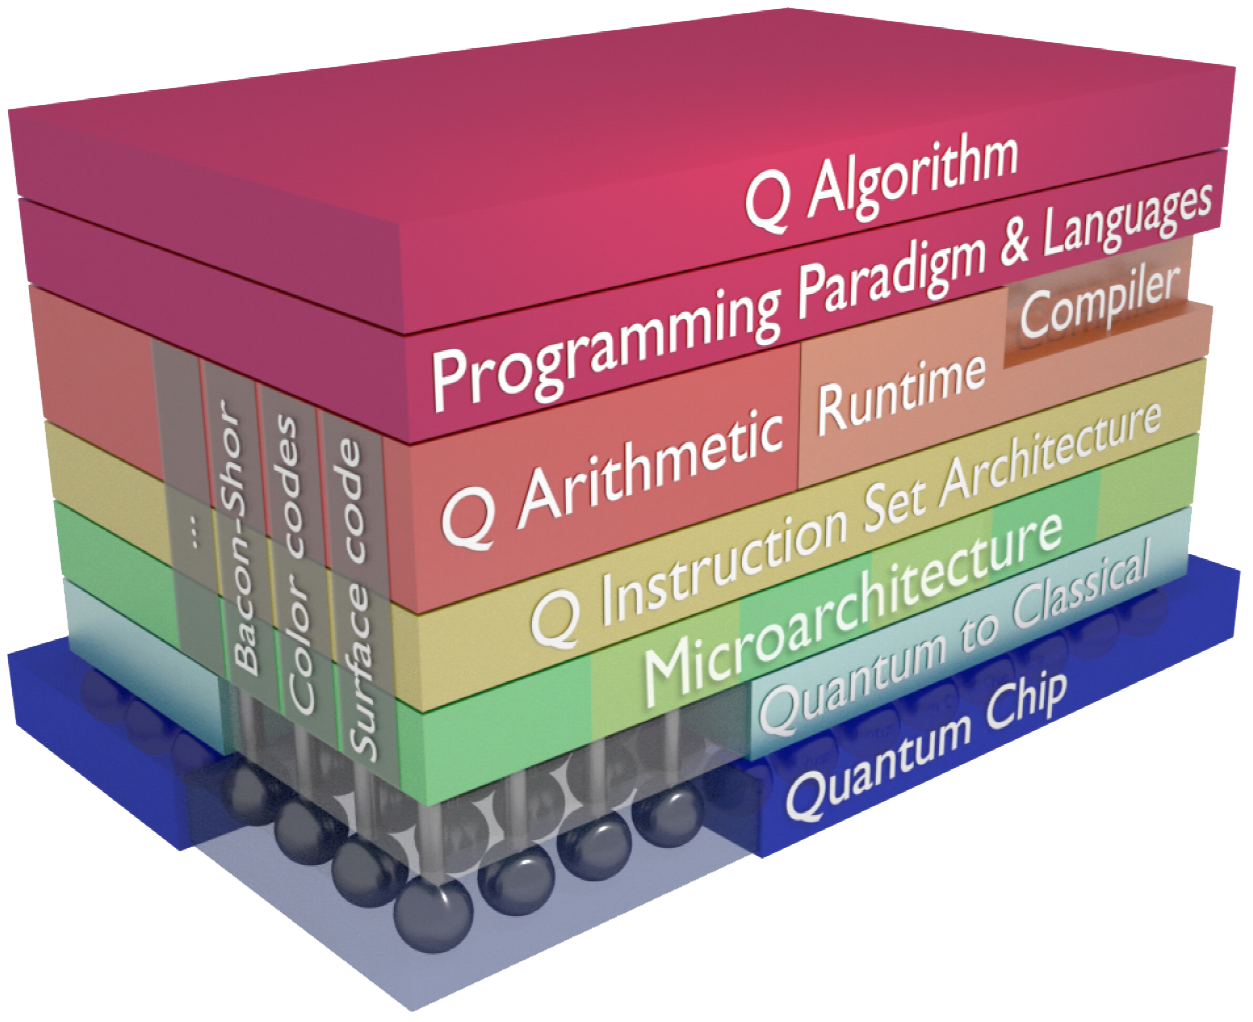
\includegraphics[width=0.7\textwidth]{figures/system_stack.png}
\caption{\label{fig:orgecea1a1}
Full stack implementation}
\end{figure}

\section{Problem Statement}
\label{sec:orgd35490c}

Quantum algorithms are represented as quantum circuits when the circuit model of computation is adopted. Quantum circuits consist of quantum bits and gates operating on them.
This representation (at high-levels of the system stack) is hardware agnostic; that is, it does not take into account the possible constraints of the quantum chip. Therefore, mapping models are required to have a version of the quantum algorithm adapted to the quantum device and that can be executed on it. 


The mapping process results in an increase of the number of gates of the circuit and/or the circuit depth (or circuit latency), affecting the reliability of the algorithm. Note that, as qubits decohere and gates are error prone, the higher the number of operations or the higher the circuit depth, the higher the probability of having an error during computation.  Therefore, mapping models require an optimization process in search of the best circuit version that is executable on a given device and still produces `good' results.

Most of the works done about the mapping task optimize in terms of two parameters, either the number of added operations in the adapted version of the circuit or the latency added to the circuit. Moreover, these works asses the quality of their mapping algorithms based on one of those two metrics. It is clear that both parameters shold be as small as possible. However, these metrics are not complete and do not tell you anything about how the mapping affects the algorithm's reliability.

Given this scenario, the aim of this thesis is two fold: i) to propose different metrics that show how the algorithm's reliability is affected by the mapping process. To this purpose, we will focus on the fidelity, the probability of success and the quantum volume; and ii) to analyze how... \textcolor{red}{Daniel, finish this sentence based on the results chapter and on what we discussed last week}

\section{Structure of the thesis}
\label{sec:org2a9c2ee}
